\documentclass[12pt, a4paper]{article}
\input{/home/mykhailo/.config/nvim/templates/preamble.tex}

\newcommand{\department}{ЗІ}
\newcommand{\reportnumber}{1}
\newcommand{\reporttitle}{Основи розробки на Python, Git та стандарти стилю коду}
\newcommand{\profname}{Кебус В. М.}

\begin{document}

\input{/home/mykhailo/Documents/lpnu/report_title_page}
Мета:
\begin{enumerate}
	\item Ознайомитися з основами роботи з розподіленою системою контролю версій Git, платформою GitHub та створенням ізольованих віртуальних середовищ (virtualenv).
	\item Навчитись створювати та структурувати проекти на Python для забезпечення багаторазового використання коду (модульність).
	\item Опанувати стандарти оформлення коду PEP-8 та навчитись перевіряти код за допомогою сучасного швидкого статичного аналізатора Ruff.
	\item Закріпити навички роботи з умовними операторами, циклами, функціями, колекціями (списки, кортежі, словники, множини), обробкою винятків та збереженням даних (CSV, JSON) у контексті прикладних задач кібербезпеки.
\end{enumerate}
\section{План виконання роботи}
\begin{enumerate}
	\item Робота з Git/GitHub: Створення репозиторію, налаштування обов'язкового віртуального середовища (virtualenv), налаштування правильної структури проєкту.
	\item Ознайомитися з правилами PEP-8: Вивчення стандартів написання якісного та читабельного коду.
	\item Налаштування аналізатора Ruff: Встановлення та інтеграція сучасного лінтера та форматизатора коду.
	\item Виконання індивідуальних завдань: Реалізація трьох комплексних завдань відповідно до свого варіанту.
	\item Аналіз коду та підготовка звіту: Перевірка написаного коду через Ruff та оформлення фінального звіту.
\end{enumerate}

\section{Завдання}
\subsection{Завдання 1: Комплексний аналізатор надійності паролів}
Реалізуйте програму, яка оцінює стійкість паролів користувача до компроментації.

\textbf{Кроки виконання:}
\begin{enumerate}
	\item Імпортуйте ваші персональні дані (ПІБ, варіант) з модуля \verb|shared/student.py|.
	\item Завантажте вихідний список паролів та критерії.
	\item Використовуючи стандартний модуль \verb|random|, згенеруйте 3 випадкові індекси зі списку паролів, візьміть відповідні паролі та додайте їх дублікати в кінець початкового списку (таким чином імітується повторне використання паролів).
	\item Оцініть надійність кожного пароля за наступним алгоритмом:

		\begin{itemize}
			\item \textbf{Заборонений: } Якщо пароль входить до списку \verb|forbidden_passwords| або його довжина менша за \verb|min_length| з критеріїв.
			\item \textbf{Слабкий: } Якщо пароль не є забороненим і виконує хоча б один з критеріїв безпеки.
			\item \textbf{Середній:} Якщо пароль відповідає мінімальній довжині та деяким (але не всім) критеріям з різних груп символів.
			\item \textbf{Сильний: } Якщо пароль відповідає абсолютно всім критеріям безпеки (довжина, цифра, велика літера, спеціальний символ), але його довжина менша за \verb|min_length + 4| символів.
			\item \textbf{Дуже сильний: } Якщо пароль відповідає всім критеріям безпеки, має довжину \verb|min_length + 4| або більше символів, та є абсолютно унікальним у всьому списку паролів.
		\end{itemize}
	\item Виведіть результат аналізу на екран у зручному табличному форматі.
\end{enumerate}

\textbf{Варіант завдання:}
\begin{lstlisting}[breaklines=true]
	passwords = ["S0cial@Engineer", "basic", "Phish1ng@D3tect", "client", "Ransomwar3@Protect", "general", "Zero@D4y", "generic", "Bug@B0untry", "standard123"]

	criteria = {"min_length": 11, "require_digits": True, "require_upper": True, "require_special": True}

	forbidden_passwords = {"basic", "client", "general", "generic", "standard123", "guest"}
\end{lstlisting}
\textbf{Виконання:}
\begin{figure}[H]
	\centering
	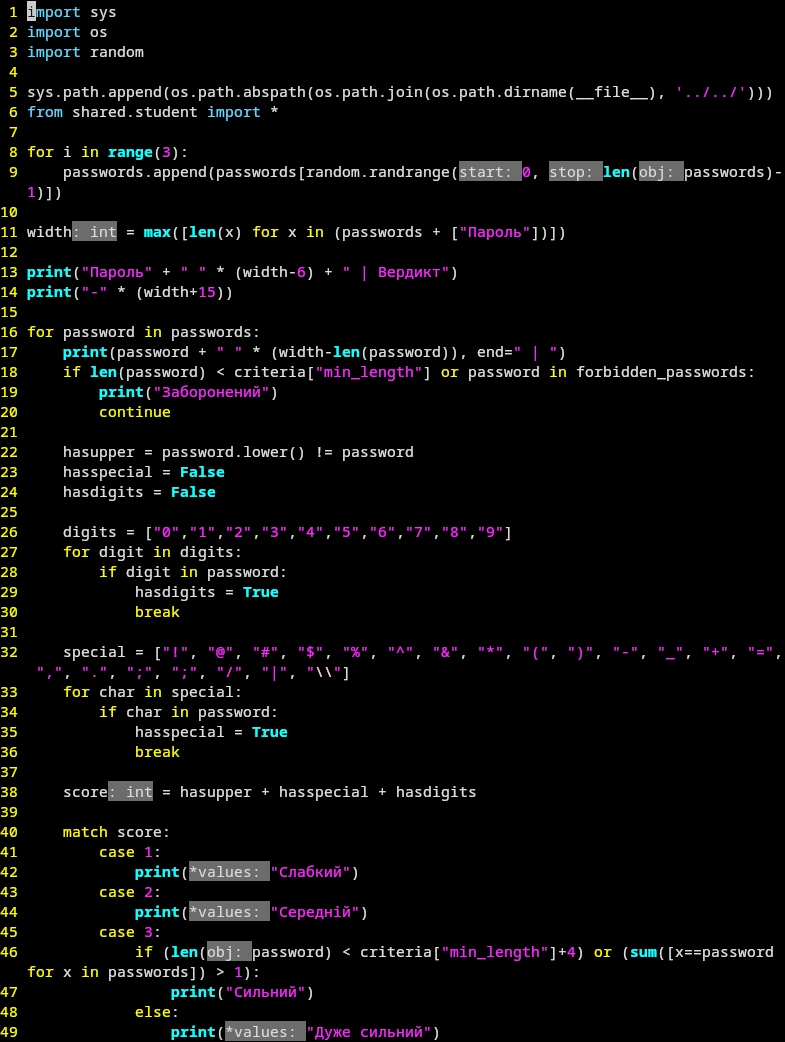
\includegraphics[width=1\textwidth]{lab1task1code.png}
	\caption{Код завдання 1}
\end{figure}
\begin{figure}[H]
	\centering
	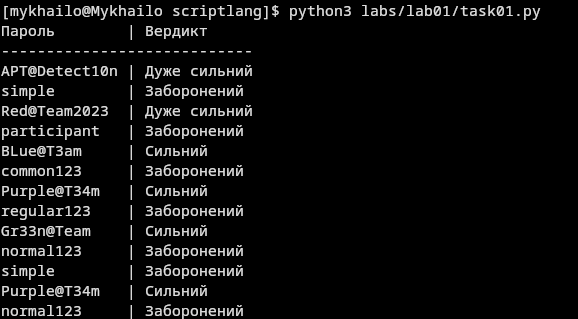
\includegraphics[width=1\textwidth]{lab1task1result.png}
	\caption{Результат виконання завдання 1}
\end{figure}
\subsection{Завдання 2: Багаторівнева система контролю доступу}
Розробіть прототип системи розмежування доступу користуачів до конфіденційних ресурcів.

\textbf{Кроки виконання:}
\begin{enumerate}
	\item Імпортуйте вхідні дані для свого варіанту (словник користувачів \verb|users|, список ресурсів \verb|resoucres|, рівні безпеки \verb|security_levels|, множину заблокованих користувачів \verb|blocked_users|).
	\item Виведіть список усіх ресурсів системи на екран, де числовий рівень безпеки  ресурсу від 1 до 4 замінено його текстовою назвою з кортежу \verb|security_levels|.
	\item Реалізуйте алгоритм перевірки доступу кожного користувача до кожного ресурсу за заданим алгоритмом:
		\begin{itemize}
			\item Якщо користувача немає в системі (словнику \verb|users|) $\rightarrow$ \textbf{DENY (User is not found)}.
			\item Якщо користувач є у списку заблокованих \verb|blocked_users| $\rightarrow$ \textbf{DENY (User is blocked)}.
			\item Якщо обліковий запис неактивний (\verb|active == False|) $\rightarrow$ \textbf{DENY (Account inactive)}.
			\item Якщо числовий рівень допуску користувача (\verb|clearance|) менший за рівень ресурсу $\rightarrow$ \textbf{DENY (Insufficient clearance)}.
			\item Якщо числовий рівень допуску користувача більший або дорівнює рівню безпеки ресурсу $\rightarrow$ \textbf{ALLOW}.
		\end{itemize}
	\item Виведіть результати перевірки на екран у форматі: \verb|user=[ім'я користувача] resource=[назва_ресурсу] ->|
		\verb|ALLOW / DENY ([причина_відмови])|
\end{enumerate}

\textbf{Варіант завдання:}
\begin{lstlisting}[breaklines=true]
	users = {
		"risk_manager": {"role": "risk_analyst", "clearance": 4, "department": "Risk Management", "active": True},

		"business_analyst": {"role": "business_analyst", "clearance": 2, "department": "Business", "active": True},

		"legal_counsel": {"role": "legal", "clearance": 3, "department": "Legal", "active": True},

		"contractor_dev": {"role": "contractor", "clearance": 2, "department": "Contractor", "active": True},

		"obsolete_system": {"role": "legacy_system", "clearance": 1, "department": "Legacy", "active": False}
	}

	resources = [("risk_registers", 4), ("business_requirements", 2), ("legal_documents", 3), ("contract_code", 2), ("governance_framework", 4), ("meeting_minutes", 1), ("regulatory_reports", 3), ("executive_dashboards", 4), ("project_specs", 2), ("public_statements", 1)]

	security_levels = ("Public", "Internal Use", "Restricted", "Highly restricted")

	blocked_users = {"obsolete_system", "contract_expired", "legal_hold"}
\end{lstlisting}
\textbf{Виконання:}
\begin{figure}[H]
	\centering
	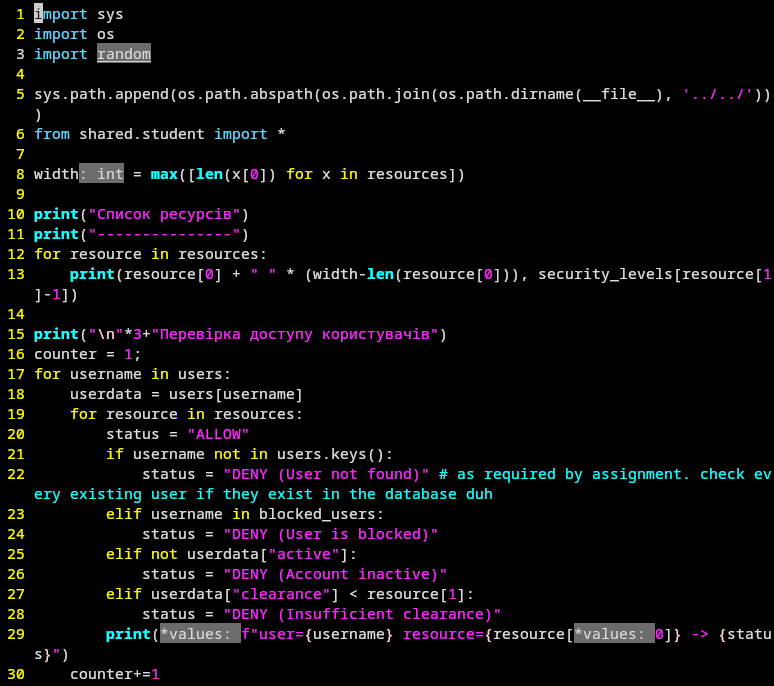
\includegraphics[width=1\textwidth]{lab1task2code.png}
	\caption{Код завдання 2}
\end{figure}
\begin{figure}[H]
	\centering
	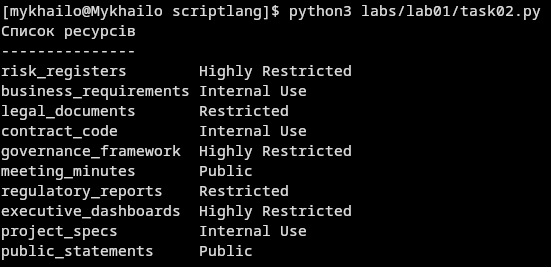
\includegraphics[width=1\textwidth]{lab1task2result.png}
	\caption{Результат виконання завдання 2 (1 з 2)}
\end{figure}
\begin{figure}[H]
	\centering
	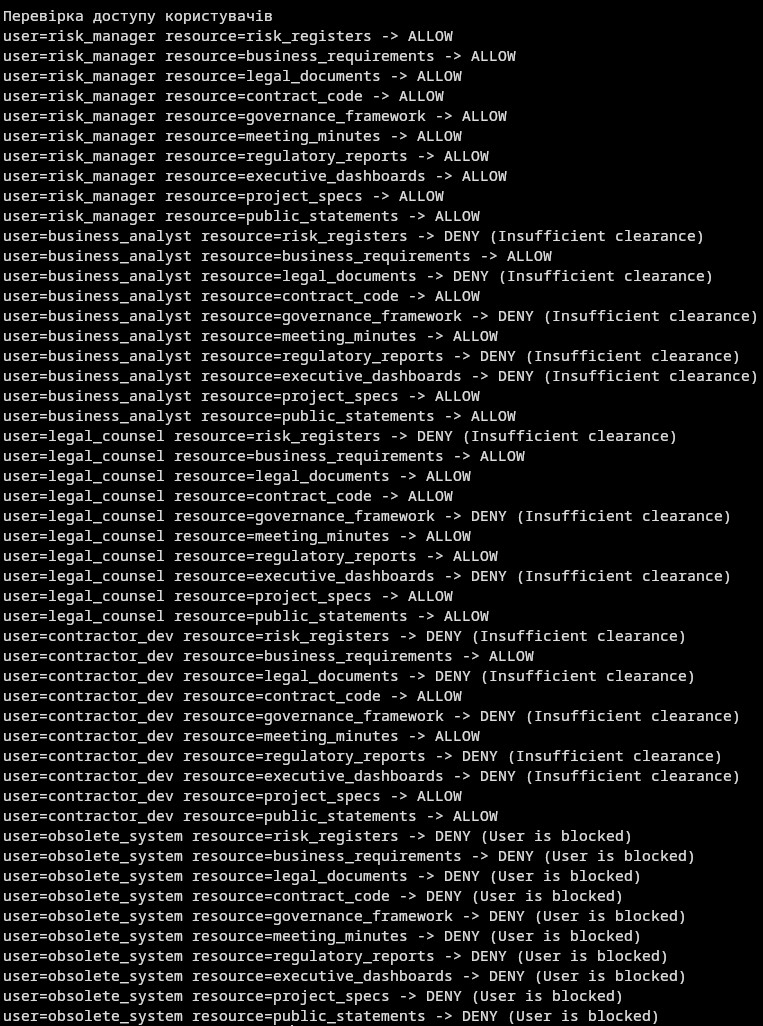
\includegraphics[width=1\textwidth]{lab1task2result2.png}
	\caption{Результат виконання завдання 2 (2 з 2)}
\end{figure}
\subsection{Завдання 3: Безпечне хешування, CVS-база та JSON-логування з винятками}
Реалізуйте модуль для безпечної реєстрації та автентифікації користувачів, використовуючи функції, декоратори та роботу з файлами.

\textbf{Кроки виконання:}
\begin{enumerate}
	\item \textbf{Хешування:} створіть функцію
	
	\verb|generate_hash(password: str, salt: str = "00000") -> str|.
		\begin{itemize}
			\item Функція має повертати шістнадцятковий хеш від конкатенації пароля та солі за допомогою алгоритму хешування з вашого варіанту.
			\item Якщо пароль або сіль порожні (\verb|None| або \verb|""|) --- згенеруйте виняток \verb|ValueError|.
			\item Якщо пароль коротший за мінімальну довжину з варіанту --- згенеруйте власний виняток \verb|ValidationError| (успадкований від \verb|Exception|).
		\end{itemize}
	\item \textbf{Персональна сіль:} створіть сіль як рядок із 5 символів, що містить ваш варіант із \verb|shared/student.py|, доповнений зліва нулями.
	\item \textbf{Реєстрація користувачів:}
		\begin{itemize}
			\item Створіть кортеж \verb|users_to_register|, що містить 10 записів у форматі \verb|(логін, пароль)|.
			\item Напишіть функцію \verb|create_user(username, password)|. Вона викликає \verb|generate_hash()| з вашою персональною сіллю та повертає кортеж \verb|(useranme, hash_value)|.
			\item Напишіть функцію \verb|create_users(users_list)| для створення бази даних. Вона обробляє весь список користувачів та записує їх у файл \verb|labs/lab01/data/users.csv| у форматі \verb|логін,хеш_пароля|.

				Переконайтеся, що папка \verb|data| створюється автоматично.
		\end{itemize}
	\item \textbf{Читання бази даних:} Зчитайте вміст CSV-файлу у список \verb|users_db| та виведіть його у вигляді структурованої таблиці на екран.
	\item \textbf{Автентифікація:} Напишіть функціюї
		\verb|login(username: str, password: str) -> bool|. 
		\begin{itemize}
			\item Перевірте, чи існує користувач у \verb|users_db| та чи збігається хеш введеного пароля (з урахуванням солі) з тим, що збережений у CSV.
			\item Якщо логін або пароль порожні --- згенеруйте \verb|ValueError|.
		\end{itemize}
	\item \textbf{Логування подій (Декоратор):} Створіть декоратор \verb|@log_event|, який записує кожну спробу входу у файл \verb|labs/lab01/data/log.json| у форматі:
		\begin{lstlisting}[breaklines=true]
			{
				"event": "login",
				"user": "username",
				"result": "success" or "failure",
				"timestamp": "YYYY-MM-DD HH:MM:SS",
				"args": [],
				"kwargs": {}
			}
		\end{lstlisting}
	\item \textbf{Обробка винятків:} Увесь код роботи з файлами та входу обгорніть у блоки \verb|try...except| із обробкою винятків: \verb|FileNotFoundError|, \verb|PermissionError|, \verb|IOError|, \verb|ValidationError| та \verb|ValueError|.
	\item Організуйте весь запуск через головну функцію \verb|main()|.
\end{enumerate}
\textbf{Виконання:}
\begin{figure}[H]
	\centering
	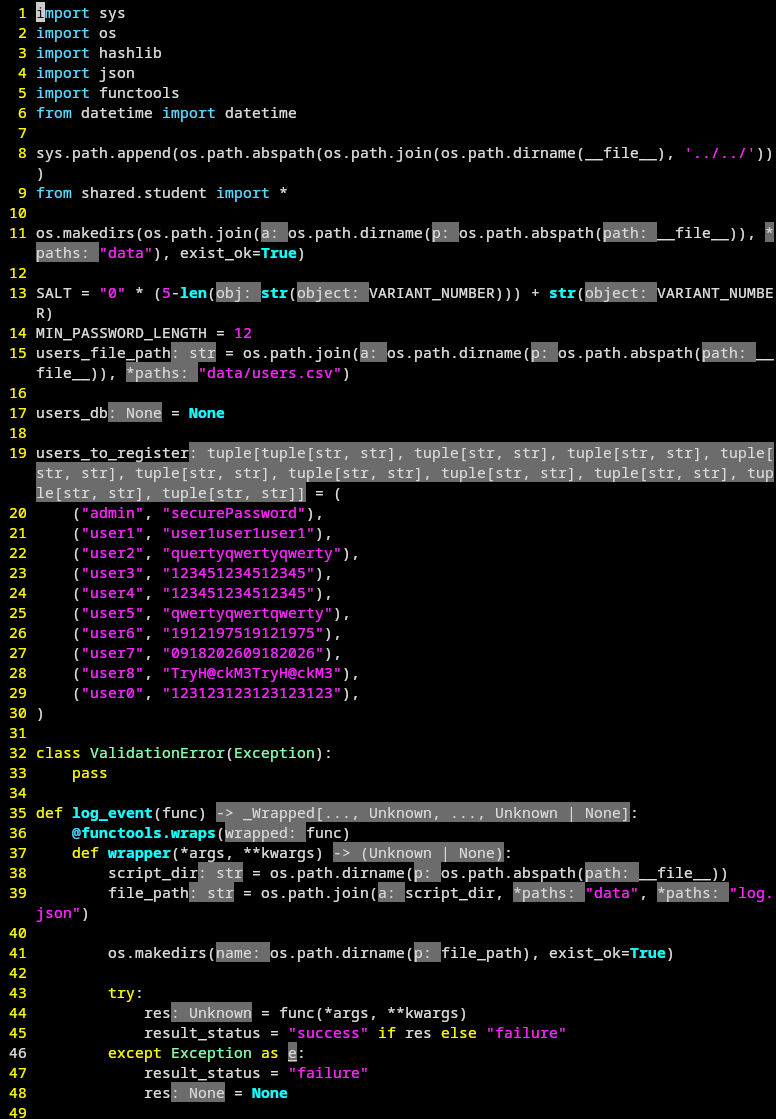
\includegraphics[width=0.8\textwidth]{lab1task3code.png}
	\caption{Код завдання 3 (1 з 3)}
\end{figure}
\begin{figure}[H]
	\centering
	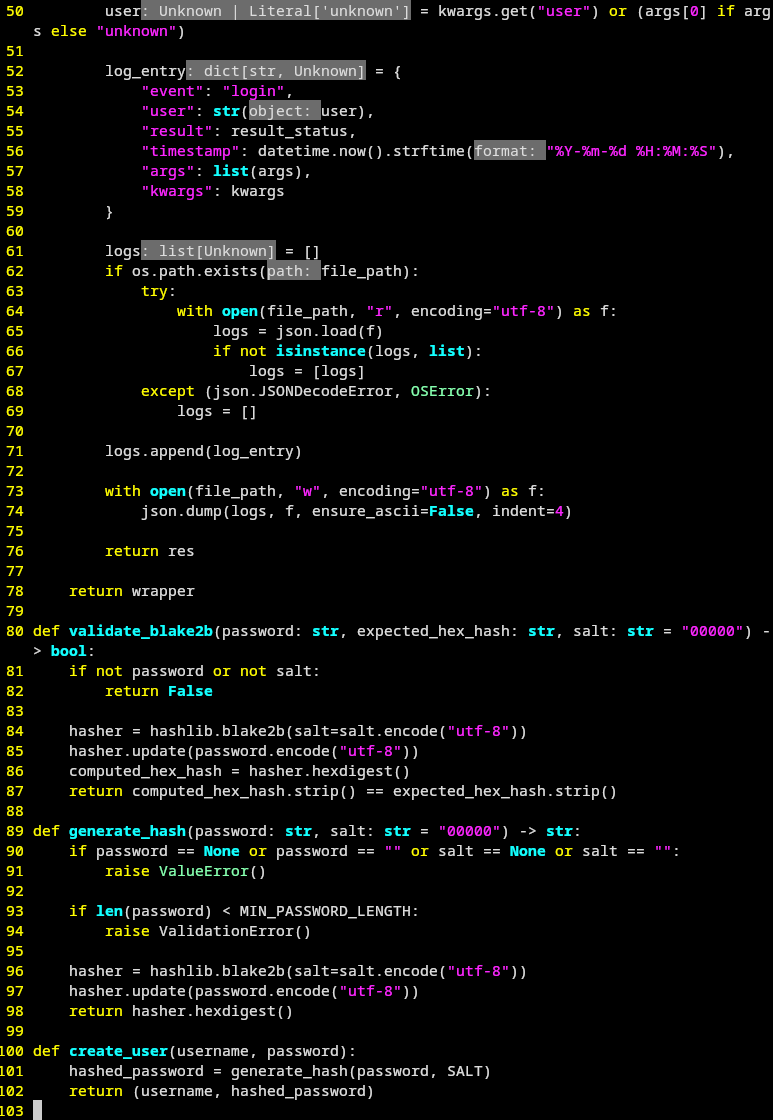
\includegraphics[width=0.8\textwidth]{lab1task3code2.png}
	\caption{Код завдання 3 (2 з 3)}
\end{figure}
\begin{figure}[H]
	\centering
	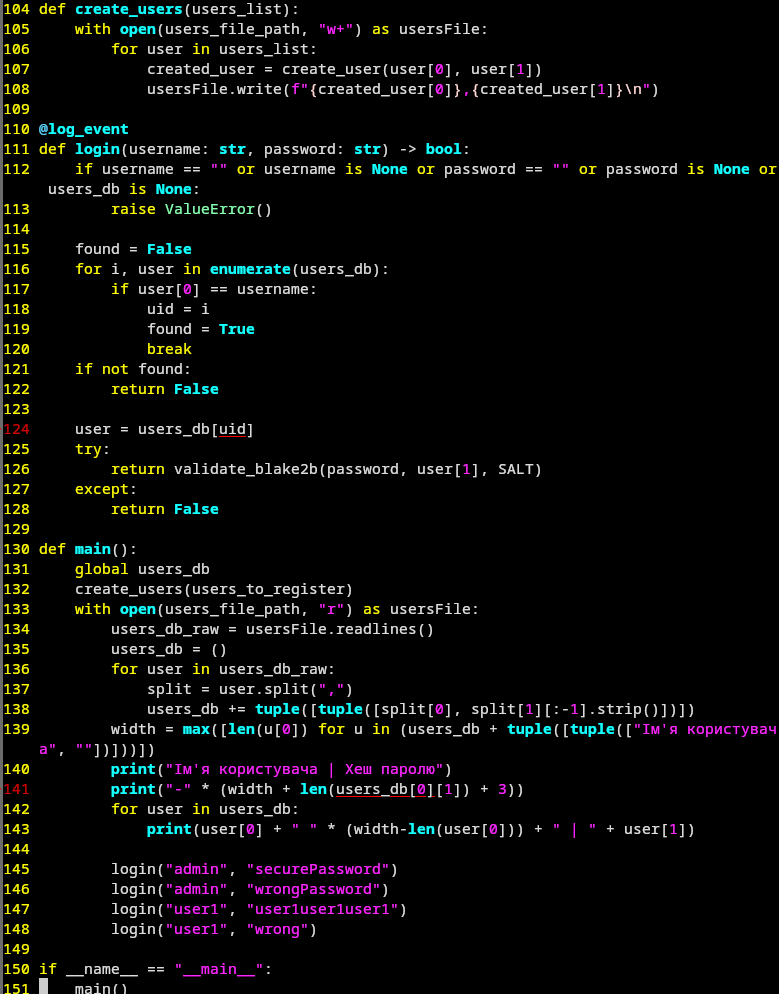
\includegraphics[width=1\textwidth]{lab1task3code3.png}
	\caption{Код завдання 3 (3 з 3)}
\end{figure}
\begin{figure}[H]
	\centering
	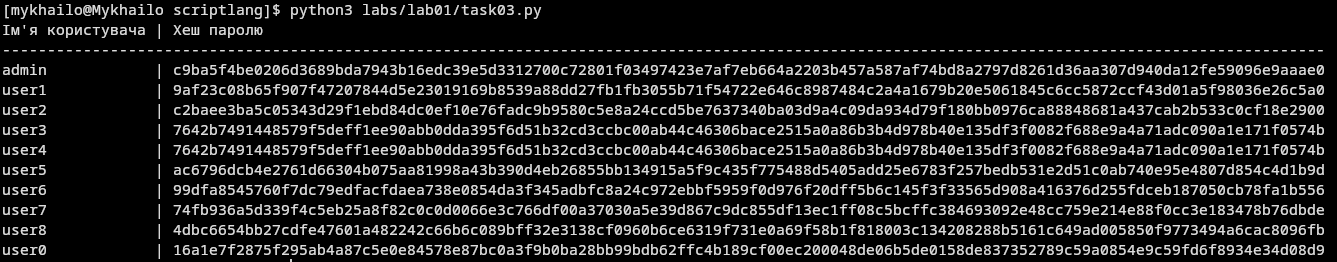
\includegraphics[width=1\textwidth]{lab1task3result.png}
	\caption{Результат виконання завдання 3}
\end{figure}
\begin{figure}[H]
	\centering
	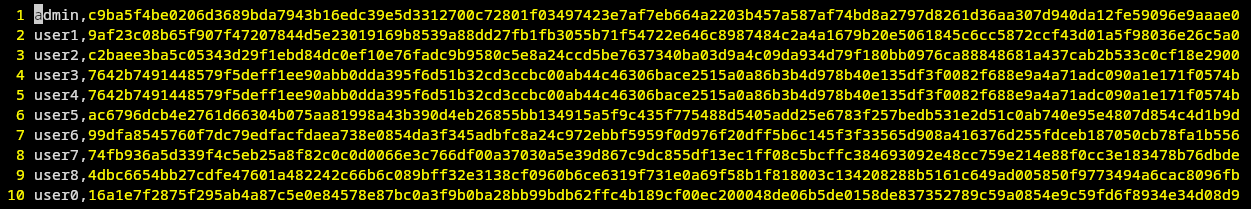
\includegraphics[width=1\textwidth]{lab1task3users.png}
	\caption{Формат файлу users.csv}
\end{figure}
\begin{figure}[H]
	\centering
	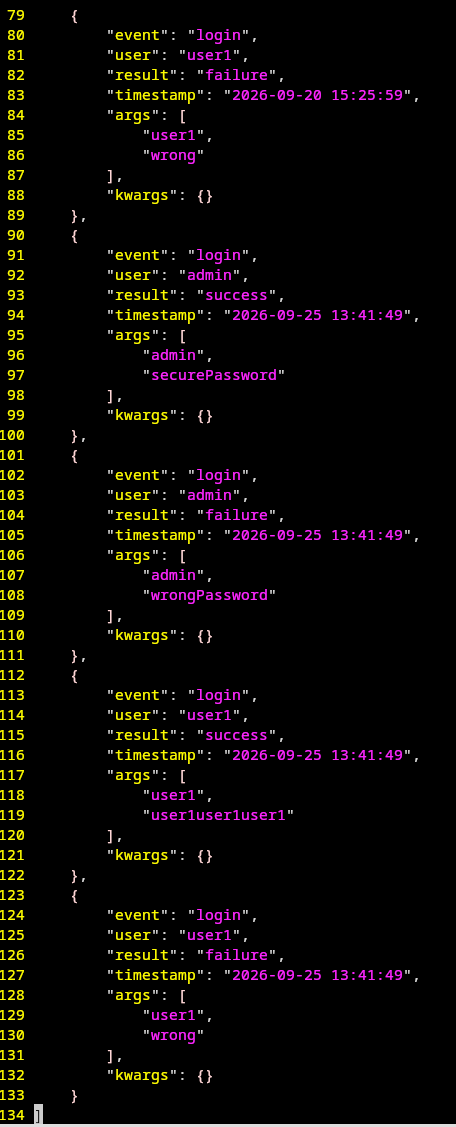
\includegraphics[width=0.5\textwidth]{lab1task3log.png}
	\caption{Формат файлу log.json}
\end{figure}
\textbf{Варіант завдання:}
\begin{itemize}
	\item Алгоритм хешування: \verb|blake2b|
	\item Мінімальна довжина пароля: 12
\end{itemize}
\section{Висновок}
Під час виконання цієї лабораторної роботи було опановано основи роботи з розподіленою системою контролю версій \verb|Git|, платформою \verb|GitHub| та створенням ізольованих віртуальних середовищ (virtualenv). Набуто досвіду створення та структурування проектів на Python для забезпечення багаторазового використання коду (модульність). Було опановано стандарти оформлення коду PEP-8 та було набуто навиків перевірки коду за допомогою сучасного швидкого статичного аналізатора Ruff. Було закріплено навички роботи з умовними операторами, циклами, функціями, колекціями (списки, кортежі, словники, множини), обробкою винятків та збереженням даних (CSV, JSON) у контексті прикладних задач кібербезпеки.
\end{document}
